
\begin{multicols}{1}

\section{Velterra}

\vspace{5mm}

\begin{center}
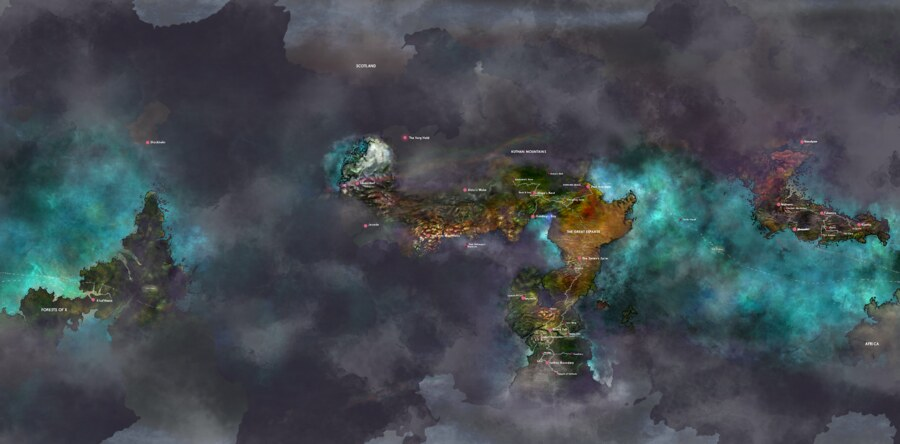
\includegraphics[width=180mm]{./content/img/velterraMap.jpg}
\begin{figure}[h]
\end{figure}
\end{center}

\end{multicols}

\begin{multicols}{2}

The year is 6653 CC (Church Calendar).  Welcome to the world of Velterra, domain of the Seven, who rule over all from afar through the constant vigilance of the Church.

Velterra is a world shaped by faith, conflict, and the long shadow of divine abandonment.  Centuries ago, the Church, believing it was protecting the world from danger, used a most powerful artefact, the Great Stone of the Eight (though you would call it Seven), to sunder the world from the gods and from the realms beyond.  The seal filters the gods' power, and the Church bends this diminished influence to its own wishes.  They had good intentions to begin with, and still believe they are doing right by the world, but they are no longer.

The world is divided into several major regions.  The Main Land, named Valeria in the old records, though almost nobody calls it that, is dominated by the Church's influence, stretching from the frozen north, where goblin tribes live under the brutal reign of the Varg warlords, to the civilised cities of the south.  Hope's Rest, the largest city in the empire, serves as the commercial and political heart of the Church-controlled territories.  Beyond the Main Land lie the continents of Nanduan and Masuda to the east, the mysterious jungles of South Africa, and the burning sands of the Great Expanse.

Magic exists in Velterra, though the Church views it with deep suspicion.  The ancient arts have been waning since the Sundering, and few practitioners remain.  The most powerful magical artefacts, the Slab of Inthun, the Stone of Unthala, the Puzzle Die of Ruh'Breks, and the star-metal known as Excalibrum, are remnants of a more powerful age, jealously guarded or lost to time.

The monetary system uses gold, silver, and copper pieces, consistent across Church-controlled territories.  Trade flows through major ports like Port Averdale and along the cobbled roads connecting the empire's cities.  Beyond Church borders, different customs and currencies prevail.

\subsection*{The Sundering}

Many centuries ago, the Church used the Great Stone to sever the world's connection to the gods and the realms beyond.  This event, known as the Sundering, was intended to protect the mortal world from external threats.  However, the centuries have not been kind.  With the gods reduced to distant, filtered influences, the Church has become corrupt, and the world is now endangered more than anything that came before.

The only hope for the souls of the world is to ``break the seal'', to unlock the gods' power and bring them back to full strength.  The Church will oppose this at all costs, but once the seal is broken, the Church will either fall or be reborn.

\subsection*{The Afterlife}

Hell exists as a bureaucratic dimension of the afterlife, managed by devils who handle the bookkeeping while demons do the torturing.  The excessive numbers of hell-bound souls, a consequence of the Church's draconian definition of sins, prompted the devil Lazarus to recruit mortal agents to bring down the Church and restore balance to the cosmic order.

Heaven, or at least the realm of the gods, has been largely inaccessible since the Sundering.  The path of ``decent and noble'' souls to their rightful rest has been corrupted by the Church's seal.

\end{multicols}

\twocolumn

\clearpage
